\documentclass[
11pt, % The default document font size, options: 10pt, 11pt, 12pt
%codirector, % Uncomment to add a codirector to the title page
]{charter} 


% El títulos de la memoria, se usa en la carátula y se puede usar el cualquier lugar del documento con el comando \ttitle
\titulo{Interfaces Cerebro-Cloud para la predicción de actividades de imaginación motriz}

% Nombre del posgrado, se usa en la carátula y se puede usar el cualquier lugar del documento con el comando \degreename
%\posgrado{Carrera de Especialización en Sistemas Embebidos} 
%\posgrado{Carrera de Especialización en Internet de las Cosas} 
\posgrado{Carrera de Especialización en Inteligencia Artificial}
%\posgrado{Maestría en Sistemas Embebidos} 
%\posgrado{Maestría en Internet de las cosas}

% Tu nombre, se puede usar el cualquier lugar del documento con el comando \authorname
% IMPORTANTE: no omitir titulaciones ni tildación en los nombres, también se recomienda escribir los nombres completos (tal cual los tienen en su documento)
\autor{Ing. Freddy Julian Riascos Salas}

% El nombre del director y co-director, se puede usar el cualquier lugar del documento con el comando \supname y \cosupname y \pertesupname y \pertecosupname
\director{Jaime Andrés Riascos Salas}
\pertenenciaDirector{pertenencia} 
\codirector{} % para que aparezca en la portada se debe descomentar la opción codirector en los parámetros de documentclass
\pertenenciaCoDirector{FIUBA}

% Nombre del cliente, quien va a aprobar los resultados del proyecto, se puede usar con el comando \clientename y \empclientename
\cliente{Xprende}
\empresaCliente{Xprendetech S.A}
 
\fechaINICIO{11 de marzo de 2025}		%Fecha de inicio de la cursada de GdP \fechaInicioName
\fechaFINALPlan{22 de abril de 2025} 	%Fecha de final de cursada de GdP
\fechaFINALTrabajo{20 de julio de 2025}	%Fecha de defensa pública del trabajo final


\begin{document}

\maketitle
\thispagestyle{empty}
\pagebreak


\thispagestyle{empty}
{\setlength{\parskip}{0pt}
\tableofcontents{}
}
\pagebreak


\section*{Registros de cambios}
\label{sec:registro}


\begin{table}[ht]
\label{tab:registro}
\centering
\begin{tabularx}{\linewidth}{@{}|c|X|c|@{}}
\hline
\rowcolor[HTML]{C0C0C0} 
Revisión & \multicolumn{1}{c|}{\cellcolor[HTML]{C0C0C0}Detalles de los cambios realizados} & Fecha      \\ \hline
0      & Creación del documento                                 &\fechaInicioName \\ \hline
%1      & Se completa hasta el punto 5 inclusive                & {día} de {mes} de 202X \\ \hline
%2      & Se completa hasta el punto 9 inclusive
%		  Se puede agregar algo más \newline
%		  En distintas líneas \newline
%		  Así                                                    & {día} de {mes} de 202X \\ \hline
%3      & Se completa hasta el punto 12 inclusive                & {día} de {mes} de 202X \\ \hline
%4      & Se completa el plan	                                 & {día} de {mes} de 202X \\ \hline

% Si hay más correcciones pasada la versión 4 también se deben especificar acá

\end{tabularx}
\end{table}

\pagebreak



\section*{Acta de constitución del proyecto}
\label{sec:acta}

\begin{flushright}
Buenos Aires, \fechaInicioName
\end{flushright}

\vspace{2cm}

Por medio de la presente se acuerda con el \authorname\hspace{1px} que su Trabajo Final de la \degreename\hspace{1px} se titulará ``\ttitle'' y consistirá en \textcolor{red}{evaluar una interfaz cerebro-computadora (Brain-Computer Interface, BCI) con soporte en la nube para la detección de patrones de imaginación motriz}. El trabajo tendrá un presupuesto preliminar estimado de \textcolor{red}{600} horas y un costo estimado de \textcolor{red}{\$ -}, con fecha de inicio el \fechaInicioName\hspace{1px} y fecha de presentación pública el \fechaFinalName.

Se adjunta a esta acta la planificación inicial.

\vfill

% Esta parte se construye sola con la información que hayan cargado en el preámbulo del documento y no debe modificarla
\begin{table}[ht]
\centering
\begin{tabular}{ccc}
\begin{tabular}[c]{@{}c@{}}Dr. Ing. Ariel Lutenberg \\ Director posgrado FIUBA\end{tabular} & \hspace{2cm} & \begin{tabular}[c]{@{}c@{}}\clientename \\ \empclientename \end{tabular} \vspace{2.5cm} \\ 
\multicolumn{3}{c}{\begin{tabular}[c]{@{}c@{}} \supname \\ Director del Trabajo Final\end{tabular}} \vspace{2.5cm} \\
\end{tabular}
\end{table}




\section{1. Descripción técnica-conceptual del proyecto a realizar}
\label{sec:descripcion}

% ELIMINAR \begin{consigna}{red} y \end{consigna}{red} en las secciones que vayan completando para cada entrega parcial.
Las interfaces cerebro-computadora (Brain-Computer Interfaces, BCI) han emergido como una tecnología innovadora que permite la comunicación directra entre el cerebro humano y dispositivos externos.
En particular, la predicción de actividades de imaginación motriz a través de BCI han cobrado relevancia en campos que varian desde la rehabilitación, robótica, control de protésis hasta sistemas domóticos, videojuegos y realidad virtual.

La integración de las BCI con tecnologías en la nube permite el almaceniamiento, procesamiento y análisis eficiente de grandes volúmenes de datos cerebrales, favoreciendo la aplicación de algoritmos avanzados de aprendizaje automático y mejorando la precisión de la interpretación de señales cerebrales.

\textbf{1.1 Conceptos Fundamentales}

\textbf{Interfaces Cerebro-Computadora}

Los BCI son sistemas que registran la actividad cerebral mediante técnicas como la electroencefalografía (EEG) y traducen estas señales en comandos computacionales. Existen distintos tipos de BCI:
\begin{itemize}
	\item \textbf{Invasivas}: Electrodos implantados directamente en el cerebro.
	\item \textbf{No invasivas}: Uso de sensores externos como EEG, MEG o fNIRS.
\end{itemize}

\textbf{Imaginación Motriz}

La imaginación motriz se refiere a la capacidad de representar mentalmente movimientos sin ejecutarlos físicamente. Durante este proceso, se activan patrones específicos en la corteza motora, los cuales pueden ser detectados mediante EEG y utilizados para el control de dispositivos externos.

\textbf{Computación en la Nube y BCI}

El uso de servicios en la nube permite procesar grandes volúmenes de datos EEG en tiempo real obteniendo beneficios como:
\begin{itemize}
	\item Almacenamiento y procesamiento escalable de datos cerebrales.
	\item Acceso remoto para análisis colaborativo.
	\item Implementación de modelos de aprendizaje automático en infraestructura distribuida.
\end{itemize}

\textbf{1.2 Problema Actual}

Al presente, las personas con discapacidades motoras severas enfrentan grandes dificultades en la interración con su entorno. Los sistemas actuales de BCI presentan limitaciones en términos de precisión, latencia, accesibilidad, recopilación,
análisis y clasificación de las señales EEG. Normalmente, estos datos se encuentran contaminados por distintos artefactos biológicos (señales cardiacas, respiratorias, músculos) como también por ruidos externos.

Así mismo, la dimensión de estos datos (n-canales x señal del tiempo) crea una problematica latente en su procesamiento eficaz de tal manera que el clasificador reciba características latentes de la señal y así realizar la predicción de forma adecuada y rápida.

\textbf{1.3 Solución Propuesta}

La interfaz Cerebro-Cloud sugerida integra un modelo de predicción basado en aprendizaje automático con una arquitectura en la nube que permita la adquisición, procesamiento y transmisión de señales cerebrales en tiempo real. Esto proporcionará una solución más precisa, escalable y accesible para el control
de dispositivos mediante imaginación motriz.



En comparación con el estado del arte actual, la solución se destaca en:

\begin{itemize}
	\item \textbf{Precisión mejorada}: Uso de modelos de inteligencia artificial optimizados para la interpretación de señales eléctricas (electroencefalografía, EEG).
	\item \textbf{Reducción de latencia}: Procesamiento distribuido en la nube.
	\item \textbf{Accesibilidad}: Plataforma escalable con acceso a la información para usuarios y especialistas.
\end{itemize}

Este interfaz BCI-Cloud tiene como objetivo mejorar la calidad de vida de personas con discapacidades motoras
al proporcionar una herramienta en la nube para la comunicación y control de dispositivos protésicos.

El proyecto se enmarca dentro de un programa de innovación tecnológica de la empresa \clientename y es financiado por la misma.

\textbf{1.4 Descripción Funcional y Diagrama en Bloques}

La solución propuesta consta de los siguientes módulos principales:
\begin{itemize}
	\item \textbf{Adquisición de Señales EEG}: Sensores no invasivos capturan la actividad cerebral del usuario.
	\item \textbf{Preprocesamiento de Datos}: Filtrado y eliminación de ruido en las señales EEG.
	\item \textbf{Modelo de Predicción}: Algoritmos de aprendizaje automático analizan los datos y determinan la intención motriz.
	\item \textbf{Transmisión en la Nube}:  Los datos procesados se envían a servidores remotos para análisis y almacenamiento.
	\item \textbf{Interfaz Usuario-Dispositivo}: Una interfaz que traduce la predicción en comandos para dispositivos externos, como prótesis o interfaces de control.
\end{itemize}

En la figura 1 se presenta el diagrama de bloques del sistema BCI-CLOUD, se observa que el usuario inicial genera datos con el sensor EEG, para luego enviar los datos a un sistema de preprocesamiento, una vez estan óptimos se envian a la nube y posteriormente el modelo seleccionado se entrena, para finalmente predecir el movimiento imaginado en la interfaz de usaurio.

\begin{figure}[htpb]
\centering 
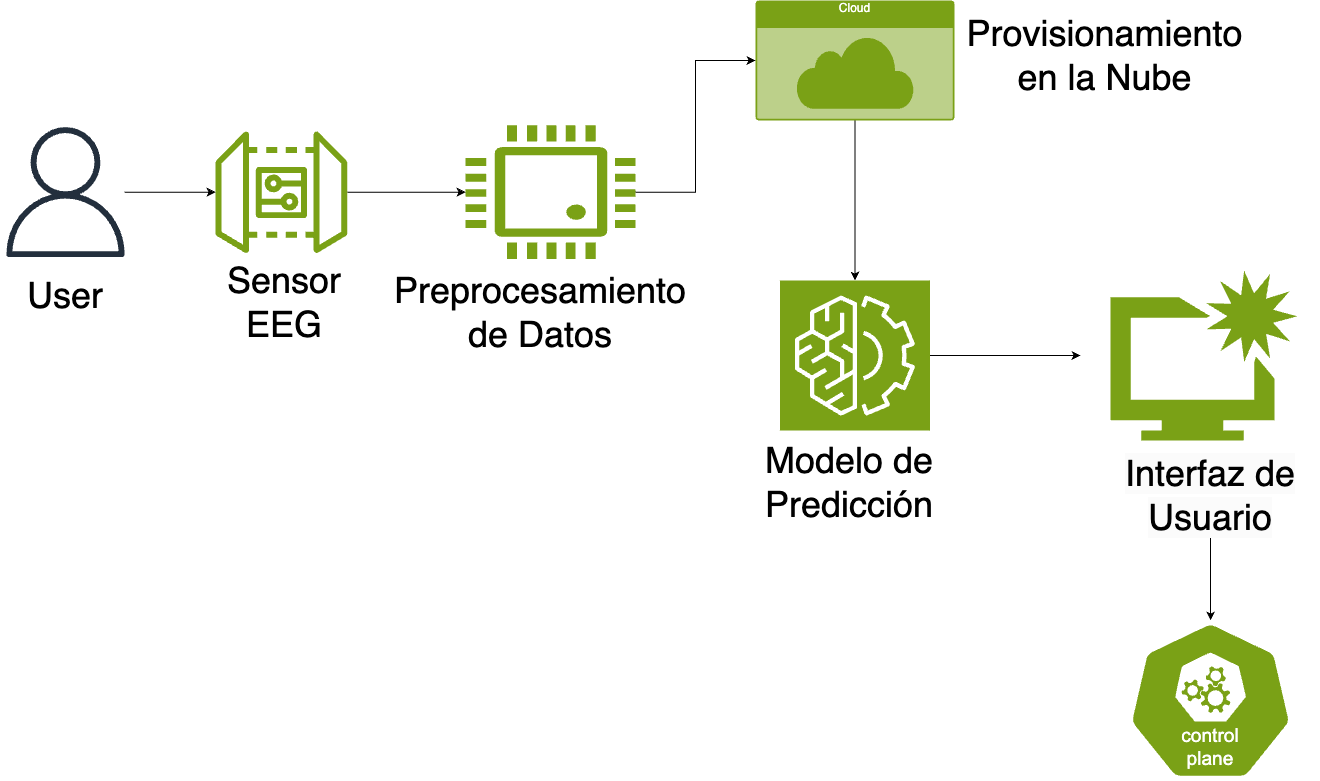
\includegraphics[width=.65\textwidth]{./Figuras/block_diagram.png}
\caption{Diagrama del sistema BCI-CLOUD.}
\label{fig:diagBloques}
\end{figure}

\vspace{25px}

% ELIMINAR \begin{consigna}{red} y \end{consigna}{red} en las secciones que vayan completando para cada entrega parcial.

\section{2. Identificación y análisis de los interesados}
\label{sec:interesados}

A continuación, se presentan los principales actores involucrados en el desarollo del proyecto y su respectiva función:
 
Es inusual que una misma persona esté en más de un rol, incluso en proyectos chicos. Si se considera que una persona cumple dos o más roles, entonces \textbf{solo dejarla en el rol más importante}. 

Por ejemplo, si una persona es Cliente pero también colabora u orienta, dejarla solo como Cliente. Si una persona es el Responsable, \textbf{no debe ser colocado también como miembro del equipo}.


\begin{table}[ht]
%\caption{Identificación de los interesados}
%\label{tab:interesados}
\begin{tabularx}{\linewidth}{@{}|l|X|X|l|@{}}
\hline
\rowcolor[HTML]{C0C0C0} 
Rol           & Nombre y Apellido & Organización 	& Puesto 	\\ \hline
Cliente       & \clientename      &\empclientename	& -       	\\ \hline
Responsable   & \authorname       & FIUBA        	& Alumno 	\\ \hline
Orientador    & \supname	      & \pertesupname 	& Director del Trabajo Final \\ \hline
Usuario final & Paciente          & -             	& -        	\\ \hline
\end{tabularx}
\end{table}

A continuación las principales características de cada interesado.
 
\begin{itemize}
	\item Orientador: Mag. Ing. Andrés Salas es experto en desarrollar interfaces cerebro-maquina y va a orientar con la definición de los requerimientos y el desarrollo del sistema BCI-Cloud.
	\item Usuario Final: Usuario con discapacidad motora severa, quien se beneficiaría directamente del control del dispositivo y la interfaz.
\end{itemize}

% ELIMINAR \begin{consigna}{red} y \end{consigna}{red} en las secciones que vayan completando para cada entrega parcial.
\section{3. Propósito del proyecto}
\label{sec:proposito}
La intención del proyecto es diseñar y desarrollar una plataforma basada en BCI-Cloud que facilite la predicción de actividades de imaginación motriz en personas con discapacidades motoras severas. A través de la integración de inteligencia artificial y computación en la nube, se busca ofrecer una solución innovadora que permita mejorar la interacción con el entorno mediante el control preciso de dispositivos electrónicos y protésicos.

\section{4. Alcance del proyecto}
\label{sec:alcance}

El proyecto comprenderá los siguientes componentes:
\begin{itemize}
	\item Modelo de predicción basado en algoritmos de aprendizaje automático para la interpretación de señales EEG. Se evaluarán distintos modelos como CNNs, RNNs y Transformers para determinar el que mejor performe en términos de precisión y latencia.
	\item Datos adquiridos de sensores EEG, los cuales se utilizarán para entrenar y validar el modelo. Se garantizará que la adquisición de datos cumpla con estándares de calidad y se preprocesen para eliminar ruido.
	\item Código de la infraestructura en la nube.
	\item Documentación técnica y científica, que detalla el diseño, implementación y validación del sistema.
	\item Pruebas y validaciones realizadas con usuarios objetivo para evaluar el desempeño y precisión del modelo. Se incluirán métricas clave que garanticen el óptimo performance del sistema.
	\item Desarrollo y entrenamiento del modelo de predicción de actividades de imaginación motriz, con comparaciones entre distintos enfoques de IA.
	\item Integración con una infraestructura en la nube escalable y segura en AWS.
	\item Adquisición y procesamiento de señales cerebrales mediante sensores EEG.
	\item Evaluación del sistema con usuarios finales para validar su precisión y usabilidad.
	\item Generación de documentación técnica para futuras mejoras e implementación.
	\item Optimización del procesamiento en la nube para reducir latencia y mejorar la eficiencia del sistema.
\end{itemize}
El presente proyecto no incluye:
\begin{itemize}
	\item Desarrollo de hardware EEG propio (se utilizarán dispositivos comerciales disponibles en el mercado).
	\item Implementación de interfaces cerebro-máquina más allá de la imaginación motriz.
	\item Integración con sistemas de salud o bases de datos clínicas.
\end{itemize}

% ELIMINAR \begin{consigna}{red} y \end{consigna}{red} en las secciones que vayan completando para cada entrega parcial.


\section{5. Supuestos del proyecto}
\label{sec:supuestos}
\begin{itemize}
	\item Disponibilidad de datos EEG de calidad: Se asume que los datos recopilados mediante sensores EEG serán suficientes y de calidad adecuada para el entrenamiento del modelo sin necesidad de un preprocesamiento excesivo.
	\item Recursos computacionales: Se cuenta con acceso a instancias de cómputo en la nube (AWS) que permitan el entrenamiento y despliegue del modelo de inteligencia artificial sin limitaciones de procesamiento o almacenamiento.
	\item Factibilidad técnica de integración: Se considera viable la integración entre los sensores EEG, la infraestructura en la nube y la interfaz de usuario.
	\item Condiciones regulatorias favorables: No existen restricciones legales o normativas que impidan la recopilación y procesamiento de datos EEG.
	\item Adopción del sistema por parte de los usuarios: Se espera que los usuarios finales (personas con discapacidades motoras) puedan adaptarse y beneficiarse de la solución sin requerir un entrenamiento extenso.
\end{itemize}

% ELIMINAR \begin{consigna}{red} y \end{consigna}{red} en las secciones que vayan completando para cada entrega parcial.

\section{6. Product backlog}
\label{sec:backlog}
\begin{enumerate}
	\item Épica 1 - Adquisición y Procesamiento de Señales EEG
	\begin{enumerate}
		\item HU1 
		
		Como ingeniero, quiero capturar señales EEG para alimentar el modelo de predicción.\newline
		
		
		Dificultad: 5
		
		Complejidad: 4 
		
		Incertidumbre: 3
		
		Suma: 12 → Story Points: 12
		
		Prioridad: 1\newline
		
		
		\item HU2
		
		Como ingeniero, quiero que las señales EEG sean filtradas y normalizadas automáticamente para mejorar la calidad del entrenamiento del modelo.\newline

		Dificultad: 4 
		
		Complejidad: 2 
		
		Incertidumbre: 2 
		
		Suma: 8 → Story Points: 8

		Prioridad: 2\newline

		
	\end{enumerate}
	\item Épica 2 - Inteligencia Artificial y Modelado
	\begin{enumerate}
		\item Como ingeniero, quiero entrenar un modelo de IA con señales EEG preprocesadas para predecir actividades de imaginación motriz con alta precisión.\newline
		
		Dificultad: 5
		
		Complejidad: 5
		
		Incertidumbre: 4
		
		Suma: 14 → Story Points: 14
		
		Prioridad: 3\newline
		
		\item Como ingeniero, quiero optimizar el modelo de IA para que el tiempo de respuesta sea menor a 5000ms, una precisión de 80\% y mejorar la experiencia del usuario.\newline
		
		Dificultad: 4
		
		Complejidad: 3
		
		Incertidumbre: 3
		
		Suma: 10 → Story Points: 10

		Prioridad: 4\newline
	\end{enumerate}
	\item Épica 3 - Infraestructura en la Nube
	\begin{enumerate}
		\item Como ingeniero, quiero que el procesamiento de datos EEG ocurra en AWS Lambda para mejorar la escalabilidad del sistema.\newline
		
		Dificultad: 5
		
		Complejidad: 4
		
		Incertidumbre: 3
		
		Suma: 12 → Story Points: 12

		Prioridad: 5\newline
		
		\item Como ingeniero, quiero una API REST para conectar los dispositivos EEG con la nube y enviar los datos en tiempo real.\newline
		
		Dificultad: 4
		
		Complejidad: 3
		
		Incertidumbre: 3
		
		Suma: 10 → Story Points: 10

		Prioridad: 6\newline
	\end{enumerate}
	\item Épica 4 - Interfaz de Usuario y Seguridad
	\begin{enumerate}
		\item Como usuario final, quiero visualizar mis señales EEG en una interfaz gráfica para entender cómo se interpretan mis actividades cerebrales.\newline
		
		Dificultad: 5
		
		Complejidad: 3
		
		Incertidumbre: 2
		
		Suma: 10 → Story Points: 10
		
		Prioridad: 7\newline
		
		\item Como ingeniero, quiero que los datos EEG sean almacenados y transmitidos de manera segura para cumplir con las normativas de privacidad."\newline
		
		Dificultad: 5
		
		Complejidad: 5
		
		Incertidumbre: 2
		
		Suma: 12 → Story Points: 12

		Prioridad: 8\newline
	\end{enumerate}
\end{enumerate}

\section{7. Criterios de aceptación de historias de usuario}
\label{sec:criteriosAceptacion}
\begin{enumerate}
	\item Épica 1 - Adquisición y Procesamiento de Señales EEG

	\begin{enumerate}
		\item Criterios de aceptación - HU1
			\begin{itemize}
				\item Se debe capturar datos EEG con una frecuencia mínima de 250 Hz.
				\item Los datos deben ser transmitidos a la nube con una latencia máxima de 5000 ms.
				\item La adquisición de datos debe ser continua y sin interrupciones durante al menos 30 minutos de prueba.
				\item Los archivos generados deben almacenarse en AWS seleccionando el mejor sistema de almacenamiento teniendo en cuenta costo y beneficio.
			\end{itemize}
			  
		\item Criterios de aceptación HU2
			\begin{itemize}
			\item Las señales EEG deben ser preprocesadas eliminando ruido y artefactos antes del almacenamiento.
			\item Los datos normalizados deben ser accesibles en una base de datos en la nube.
			\item  La precisión del filtrado debe validarse con al menos un 95\% de efectividad en la eliminación de ruido.
			\end{itemize}
	\end{enumerate}
	\item Épica 2 - Inteligencia Artificial y Modelado
	\begin{enumerate}
		\item Criterios de aceptación HU3
			\begin{itemize}
			\item  El modelo de predicción debe alcanzar una precisión mínima del 85\% en validación cruzada.
			\item  Se deben entrenar al menos tres arquitecturas y seleccionar la mejor.
			\item  Se deben generar logs detallados del proceso de entrenamiento con métricas de desempeño.
			\end{itemize}
		\item Criterios de aceptación HU4
			\begin{itemize}
			\item  El modelo optimizado debe tener un tiempo de inferencia menor a 5000 ms.
			\item  La implementación debe utilizar hardware optimizado en la nube.
			\item  Se debe medir la latencia en diferentes condiciones de carga y garantizar estabilidad.
			\item Los resultados de predicción deben ser accesibles en tiempo real a través de una API.
			\end{itemize}
	\end{enumerate}
	\item Épica 3 - Infraestructura en la Nube
	\begin{enumerate}
		\item Criterios de aceptación HU5
			\begin{itemize}
			\item  La infraestructura debe ser escalable, permitiendo hasta 1000 eventos concurrentes.
			\item  Se debe garantizar un 85.9\% de disponibilidad del servicio en producción.
			\item  AWS Lambda debe procesar eventos EEG en tiempo real con ejecución máxima de 15 segundos.
			\end{itemize}
		\item Criterios de aceptación HU6
			\begin{itemize}
			\item  La API REST debe permitir la recepción de datos EEG con un endpoint dedicado.
			\item  Debe incluir autenticación y autorización mediante tokens JWT.
			\item  La API debe responder con código 200 OK en menos de 300 ms en condiciones normales.
			\item La documentación de la API debe estar disponible con ejemplos de uso.
			\end{itemize}
	\end{enumerate}
	\item Épica 4 - Interfaz de Usuario y Seguridad
	\begin{enumerate}
		\item Criterios de aceptación HU7
			\begin{itemize}
			\item La interfaz debe permitir visualizar las señales EEG en gráficos.
			\item Se debe permitir la exportación de datos en formatos CSV y JSON.
			\end{itemize}
		\item Criterios de aceptación HU8
			\begin{itemize}
			\item Los datos EEG deben ser cifrados en tránsito y en reposo.
			\item El sistema debe incluir una política de retención y eliminación de datos.
			\end{itemize}
	\end{enumerate}
\end{enumerate}

\section{8. Fases de CRISP-DM}
\label{sec:entregables}

\begin{consigna}{red}
En esta sección debe definir las 6 fases de la metodología CRISP-DM. Se pueden ayudar con las siguientes preguntas de guía:

\begin{enumerate}
	\item Comprensión del negocio.
	¿Qué objetivo se intenta cumplir? ¿Qué valor agrega la implementación de IA al problema del 			negocio? ¿Cuáles son las métricas de éxito que se utilizarán para medir el impacto del 				producto o servicio?
	\item Comprensión de los datos
	¿Con qué tipo de datos se trabajará? ¿Cuáles son las fuentes? ¿Qué cantidad? ¿Qué podría 				decir acerca de su calidad?
	\item Preparación de los datos 
	¿Cuáles consideras que son las características clave? ¿Qué tipo de transformaciones serán 				necesarias aplicar?
	\item Modelado 
	¿Qué tipo de problema se busca resolver? ¿Clasificación? ¿Predicción? ¿Qué arquitecturas 				podrían utilizarse?
	\item Evaluación del modelo 
	¿Con qué métricas se evaluará el desempeño del modelo?
	\item Despliegue del modelo [opcional]
	¿Qué tipo de despliegue se llevará a cabo? ¿Con qué herramientas? 
\end{enumerate}
La fase 6 es opcional ya que es posible que aún no cuenten con los conocimientos necesarios para definirla.
\end{consigna}

\section{9. Desglose del trabajo en tareas}
\label{sec:wbs}

\begin{consigna}{red}
El WBS debe tener relación directa o indirecta con los requerimientos.  Son todas las actividades que se harán en el proyecto para dar cumplimiento a los requerimientos. Se recomienda mostrar el WBS mediante una lista indexada:

\begin{enumerate}
\item Grupo de tareas 1 (suma h)
	\begin{enumerate}
	\item Tarea 1 (tantas h)
	\item Tarea 2 (tantas h)
	\item Tarea 3 (tantas h)
	\end{enumerate}
\item Grupo de tareas 2 (suma h)
	\begin{enumerate}
	\item Tarea 1 (tantas h)
	\item Tarea 2 (tantas h)
	\item Tarea 3 (tantas h)
	\end{enumerate}
\item Grupo de tareas 3 (suma h)
	\begin{enumerate}
	\item Tarea 1 (tantas h)
	\item Tarea 2 (tantas h)
	\item Tarea 3 (tantas h)
	\item Tarea 4 (tantas h)
	\item Tarea 5 (tantas h)
	\end{enumerate}
\end{enumerate}

Cantidad total de horas: tantas.

\textbf{¡Importante!:} la unidad de horas es h y va separada por espacio del número. Es incorrecto escribir ``23hs".

\textbf{Se recomienda que no haya ninguna tarea que lleve más de 40 h.} De ser así se recomienda dividirla en tareas de menor duración.

\end{consigna}

\section{10. Diagrama de Activity On Node}
\label{sec:AoN}

\begin{consigna}{red}
Armar el AoN a partir del WBS definido en la etapa anterior.

Una herramienta simple para desarrollar los diagramas es el Draw.io (\url{https://app.diagrams.net/}).
\href{https://app.diagrams.net}{Draw.io}


\begin{figure}[htpb]
\centering 
\includegraphics[width=.8\textwidth]{./Figuras/AoN.png}
\caption{Diagrama de \textit{Activity on Node}.}
\label{fig:AoN}
\end{figure}

Indicar claramente en qué unidades están expresados los tiempos.
De ser necesario indicar los caminos semi críticos y analizar sus tiempos mediante un cuadro.
Es recomendable usar colores y un cuadro indicativo describiendo qué representa cada color.

\end{consigna}

\section{11. Diagrama de Gantt}
\label{sec:gantt}

\begin{consigna}{red}
Existen muchos programas y recursos \textit{online} para hacer diagramas de Gantt, entre los cuales destacamos:

\begin{itemize}
\item Planner
\item GanttProject
\item Trello + \textit{plugins}. En el siguiente link hay un tutorial oficial: \\ \url{https://blog.trello.com/es/diagrama-de-gantt-de-un-proyecto}
\item Creately, herramienta online colaborativa. \\\url{https://creately.com/diagram/example/ieb3p3ml/LaTeX}
\item Se puede hacer en latex con el paquete \textit{pgfgantt}\\ \url{http://ctan.dcc.uchile.cl/graphics/pgf/contrib/pgfgantt/pgfgantt.pdf}
\end{itemize}

Pegar acá una captura de pantalla del diagrama de Gantt, cuidando que la letra sea suficientemente grande como para ser legible. 
Si el diagrama queda demasiado ancho, se puede pegar primero la ``tabla'' del Gantt y luego pegar la parte del diagrama de barras del diagrama de Gantt.

Configurar el software para que en la parte de la tabla muestre los códigos del EDT (WBS).\\
Configurar el software para que al lado de cada barra muestre el nombre de cada tarea.\\
Revisar que la fecha de finalización coincida con lo indicado en el Acta Constitutiva.

En la figura \ref{fig:gantt}, se muestra un ejemplo de diagrama de gantt realizado con el paquete de \textit{pgfgantt}. 
En la plantilla pueden ver el código que lo genera y usarlo de base para construir el propio.

Las fechas pueden ser calculadas utilizando alguna de las herramientas antes citadas. Sin embargo, el siguiente ejemplo
fue elaborado utilizando 
\href{https://docs.google.com/spreadsheets/d/1fBz8NhSpc4tkkhz3KjJCbh1nR_ltDkfEcZi4tZXduqs}{esta hoja de cálculo}.

Es importante destacar que el ancho del diagrama estará dado por la longitud del texto utilizado para las tareas 
(Ejemplo: tarea 1, tarea 2, etcétera) y el valor \textit{x unit}. Para mejorar la apariencia del diagrama, es necesario
ajustar este valor y, quizás, acortar los nombres de las tareas.

\begin{figure}[htpb]
  \begin{center}
    \begin{ganttchart}[
      time slot unit=day,
      time slot format=isodate,
      x unit=0.038cm,
      y unit title=0.7cm,
      y unit chart=0.6cm,
      milestone/.append style={xscale=4}
      ]{2021-03-05}{2021-12-16}
      \gantttitlecalendar*{2021-03-05}{2021-12-16}{year} \\
      \gantttitlecalendar*{2021-03-05}{2021-12-16}{month} \\
      \ganttgroup{Duración Total}{2021-03-05}{2021-12-16} \\
      %%%%%%%%%%%%%%%%%Organización
      \ganttgroup{Organización}{2021-03-05}{2021-04-16} \\
      \ganttbar{Planificación del proyecto}{2021-03-05}{2021-04-15} \\
      %%%%%%%%%%%%%%%%%Ejecución
      \ganttgroup{Ejecución}{2021-04-16}{2021-10-21} \\
      \ganttbar{Tarea 1}{2021-04-16}{2021-04-29} \\
      \ganttbar{Tarea 2}{2021-04-30}{2021-05-13} \\
      \ganttbar{Tarea 3}{2021-05-14}{2021-05-27} \\
      \ganttbar{Tarea 4}{2021-05-28}{2021-07-12} \\
      \ganttbar{Tarea 5}{2021-07-13}{2021-08-09} \\
      \ganttbar{Tarea 6}{2021-08-10}{2021-09-23} \\
      \ganttbar{Tarea 7}{2021-09-24}{2021-09-30} \\
      \ganttbar{Tarea 8}{2021-10-01}{2021-10-14} \\
      \ganttbar{Tarea 9}{2021-10-15}{2021-10-21} \\
      % %%%%%%%%%%%%%%%%%Finalización
      \ganttgroup{Finalización}{2021-10-22}{2021-12-16} \\
      \ganttbar{Memoria v1}{2021-10-22}{2021-11-04} \\
      \ganttbar{Memoria v2}{2021-11-05}{2021-11-18} \\
      \ganttbar{Memoria final}{2021-11-19}{2021-12-02} \\
      % La fecha del siguiente milestone es la fecha en que terminamos la memoria
      \ganttmilestone{Enviar memoria al director}{2021-12-02} \\
      \ganttbar{Elaborar la presentación}{2021-12-03}{2021-12-16} \\
      \ganttmilestone{Ensayo de la presentación}{2021-12-16} \\
      %%%%%%%%%%%%%%%%%%%%%%%%%%%%%%%%%%%%%%%%%%%%%%%%%%%%%%%%%%%%%%%
    \end{ganttchart}
  \end{center}
  \caption{Diagrama de gantt de ejemplo}
  \label{fig:gantt}
\end{figure}


\begin{landscape}
\begin{figure}[htpb]
\centering 
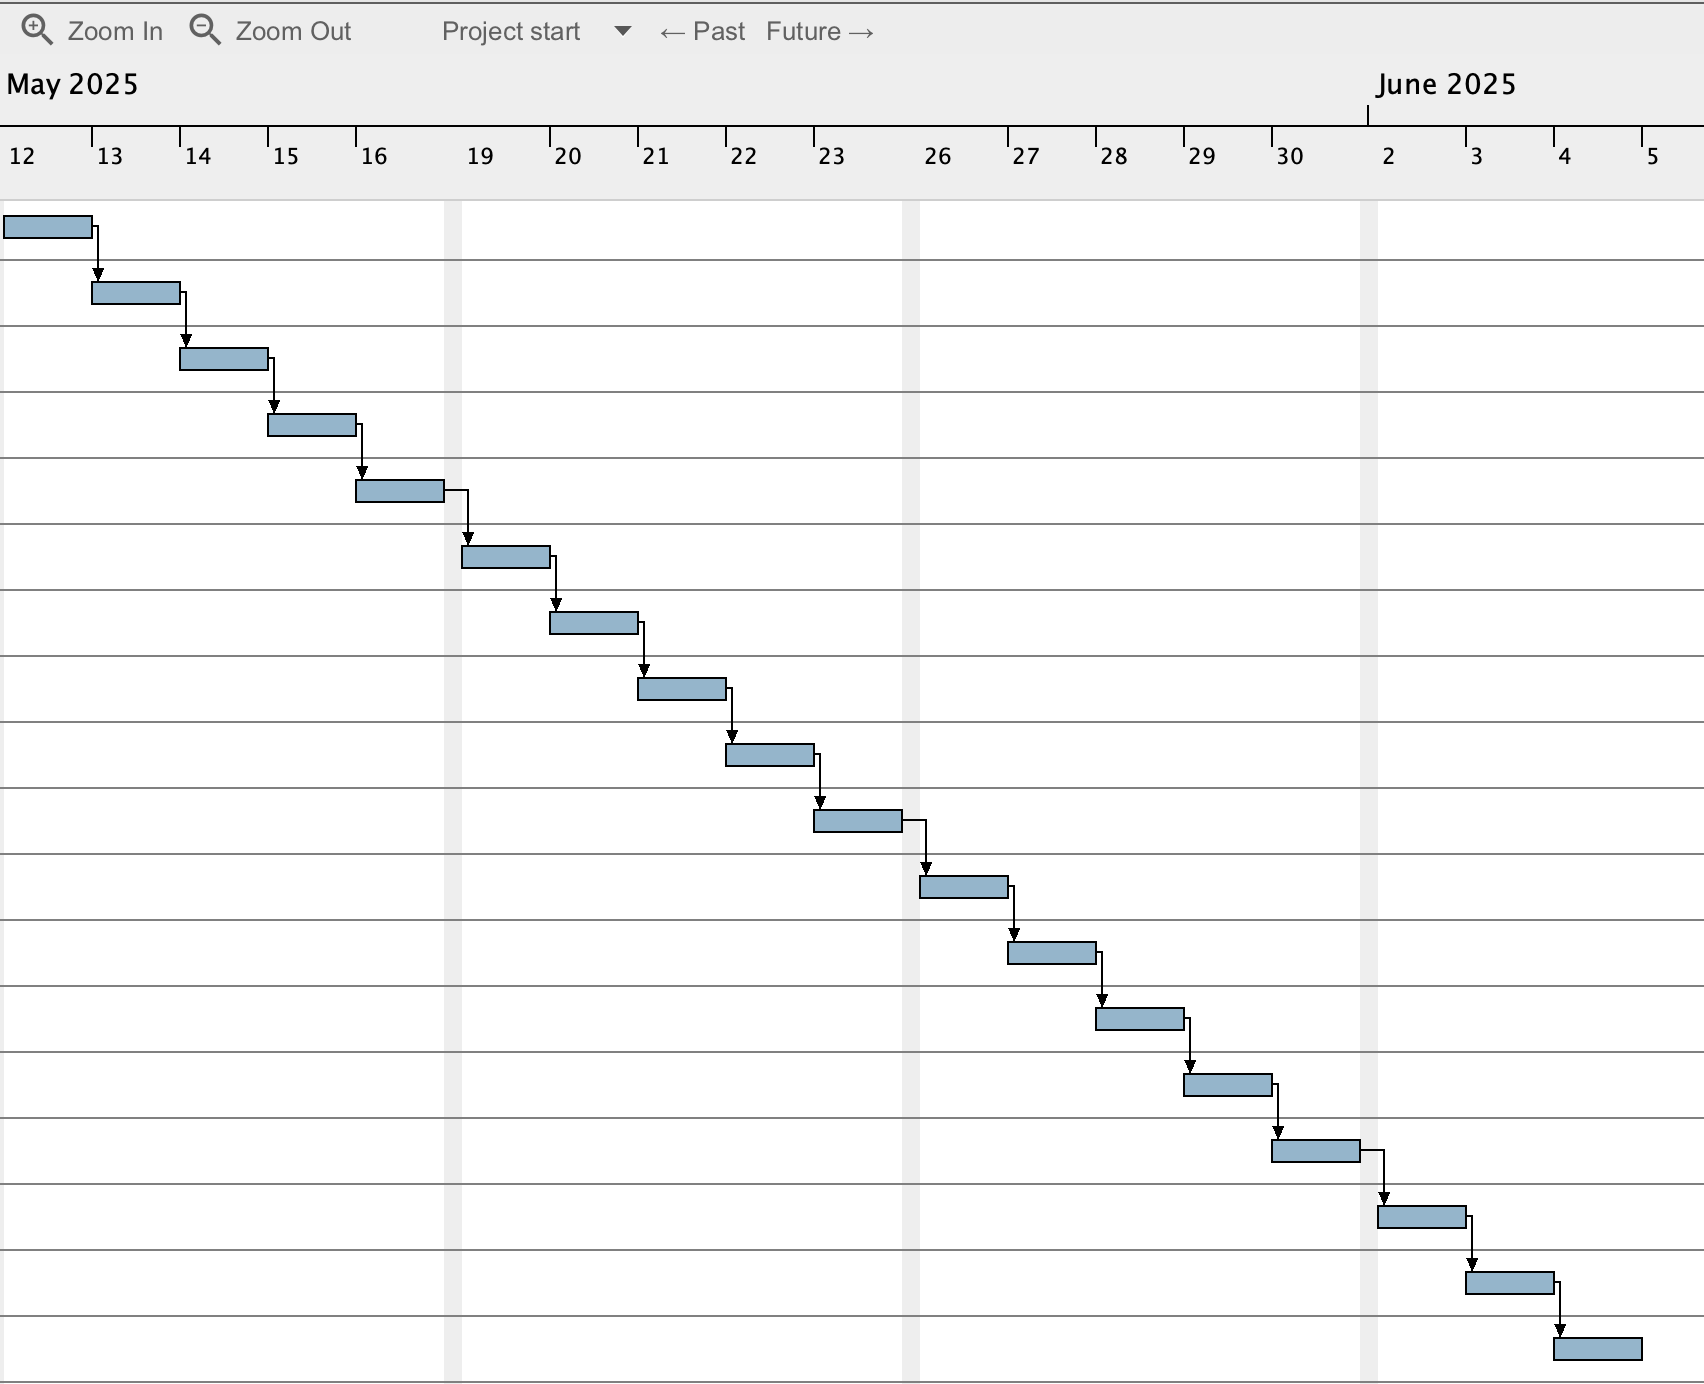
\includegraphics[height=.85\textheight]{./Figuras/Gantt-2.png}
\caption{Ejemplo de diagrama de Gantt (apaisado).} %Modificar este título acorde.
\label{fig:diagGantt}
\end{figure}

\end{landscape}

\end{consigna}


\section{12. Presupuesto detallado del proyecto}
\label{sec:presupuesto}

\begin{consigna}{red}
Si el proyecto es complejo entonces separarlo en partes:
\begin{itemize}
	\item Un total global, indicando el subtotal acumulado por cada una de las áreas.
	\item El desglose detallado del subtotal de cada una de las áreas.
\end{itemize}

IMPORTANTE: No olvidarse de considerar los COSTOS INDIRECTOS.

Incluir la aclaración de si se emplea como moneda el peso argentino (ARS) o si se usa moneda extranjera (USD, EUR, etc). Si es en moneda extranjera se debe indicar la tasa de conversión respecto a la moneda local en una fecha dada.

\end{consigna}

\begin{table}[htpb]
\centering
\begin{tabularx}{\linewidth}{@{}|X|c|r|r|@{}}
\hline
\rowcolor[HTML]{C0C0C0} 
\multicolumn{4}{|c|}{\cellcolor[HTML]{C0C0C0}COSTOS DIRECTOS} \\ \hline
\rowcolor[HTML]{C0C0C0} 
Descripción &
  \multicolumn{1}{c|}{\cellcolor[HTML]{C0C0C0}Cantidad} &
  \multicolumn{1}{c|}{\cellcolor[HTML]{C0C0C0}Valor unitario} &
  \multicolumn{1}{c|}{\cellcolor[HTML]{C0C0C0}Valor total} \\ \hline
 &
  \multicolumn{1}{c|}{} &
  \multicolumn{1}{c|}{} &
  \multicolumn{1}{c|}{} \\ \hline
 &
  \multicolumn{1}{c|}{} &
  \multicolumn{1}{c|}{} &
  \multicolumn{1}{c|}{} \\ \hline
\multicolumn{1}{|l|}{} &
   &
   &
   \\ \hline
\multicolumn{1}{|l|}{} &
   &
   &
   \\ \hline
\multicolumn{3}{|c|}{SUBTOTAL} &
  \multicolumn{1}{c|}{} \\ \hline
\rowcolor[HTML]{C0C0C0} 
\multicolumn{4}{|c|}{\cellcolor[HTML]{C0C0C0}COSTOS INDIRECTOS} \\ \hline
\rowcolor[HTML]{C0C0C0} 
Descripción &
  \multicolumn{1}{c|}{\cellcolor[HTML]{C0C0C0}Cantidad} &
  \multicolumn{1}{c|}{\cellcolor[HTML]{C0C0C0}Valor unitario} &
  \multicolumn{1}{c|}{\cellcolor[HTML]{C0C0C0}Valor total} \\ \hline
\multicolumn{1}{|l|}{} &
   &
   &
   \\ \hline
\multicolumn{1}{|l|}{} &
   &
   &
   \\ \hline
\multicolumn{1}{|l|}{} &
   &
   &
   \\ \hline
\multicolumn{3}{|c|}{SUBTOTAL} &
  \multicolumn{1}{c|}{} \\ \hline
\rowcolor[HTML]{C0C0C0}
\multicolumn{3}{|c|}{TOTAL} &
   \\ \hline
\end{tabularx}%
\end{table}


\section{13. Gestión de riesgos}
\label{sec:riesgos}

\begin{consigna}{red}
a) Identificación de los riesgos (al menos cinco) y estimación de sus consecuencias:
 
Riesgo 1: detallar el riesgo (riesgo es algo que si ocurre altera los planes previstos de forma negativa)
\begin{itemize}
	\item Severidad (S): mientras más severo, más alto es el número (usar números del 1 al 10).\\
	Justificar el motivo por el cual se asigna determinado número de severidad (S).
	\item Probabilidad de ocurrencia (O): mientras más probable, más alto es el número (usar del 1 al 10).\\
	Justificar el motivo por el cual se asigna determinado número de (O). 
\end{itemize}   

Riesgo 2:
\begin{itemize}
	\item Severidad (S): X.\\
	Justificación...
	\item Ocurrencia (O): Y.\\
	Justificación...
\end{itemize}

Riesgo 3:
\begin{itemize}
	\item Severidad (S):  X.\\
	Justificación...
	\item Ocurrencia (O): Y.\\
	Justificación...
\end{itemize}


b) Tabla de gestión de riesgos:      (El RPN se calcula como RPN=SxO)

\begin{table}[htpb]
\centering
\begin{tabularx}{\linewidth}{@{}|X|c|c|c|c|c|c|@{}}
\hline
\rowcolor[HTML]{C0C0C0} 
Riesgo & S & O & RPN & S* & O* & RPN* \\ \hline
       &   &   &     &    &    &      \\ \hline
       &   &   &     &    &    &      \\ \hline
       &   &   &     &    &    &      \\ \hline
       &   &   &     &    &    &      \\ \hline
       &   &   &     &    &    &      \\ \hline
\end{tabularx}%
\end{table}

Criterio adoptado: 

Se tomarán medidas de mitigación en los riesgos cuyos números de RPN sean mayores a...

Nota: los valores marcados con (*) en la tabla corresponden luego de haber aplicado la mitigación.

c) Plan de mitigación de los riesgos que originalmente excedían el RPN máximo establecido:
 
Riesgo 1: plan de mitigación (si por el RPN fuera necesario elaborar un plan de mitigación).
  Nueva asignación de S y O, con su respectiva justificación:
  \begin{itemize}
	\item Severidad (S*): mientras más severo, más alto es el número (usar números del 1 al 10).
          Justificar el motivo por el cual se asigna determinado número de severidad (S).
	\item Probabilidad de ocurrencia (O*): mientras más probable, más alto es el número (usar del 1 al 10).
          Justificar el motivo por el cual se asigna determinado número de (O).
	\end{itemize}

Riesgo 2: plan de mitigación (si por el RPN fuera necesario elaborar un plan de mitigación).
 
Riesgo 3: plan de mitigación (si por el RPN fuera necesario elaborar un plan de mitigación).

\end{consigna}


\section{14. Gestión de la calidad}
\label{sec:calidad}

\begin{consigna}{red}
Elija al menos diez requerimientos que a su criterio sean los más importantes/críticos/que aportan más valor y para cada uno de ellos indique las acciones de verificación y validación que permitan asegurar su cumplimiento.

\begin{itemize} 
\item Req \#1: copiar acá el requerimiento con su correspondiente número.

\begin{itemize}
	\item Verificación para confirmar si se cumplió con lo requerido antes de mostrar el sistema al cliente. Detallar.
	\item Validación con el cliente para confirmar que está de acuerdo en que se cumplió con lo requerido. Detallar. 
\end{itemize}

\end{itemize}

Tener en cuenta que en este contexto se pueden mencionar simulaciones, cálculos, revisión de hojas de datos, consulta con expertos, mediciones, etc.  

Las acciones de verificación suelen considerar al entregable como ``caja blanca'', es decir se conoce en profundidad su funcionamiento interno.  

En cambio, las acciones de validación suelen considerar al entregable como ``caja negra'', es decir, que no se conocen los detalles de su funcionamiento interno.

\end{consigna}

\section{15. Procesos de cierre}    
\label{sec:cierre}

\begin{consigna}{red}
Establecer las pautas de trabajo para realizar una reunión final de evaluación del proyecto, tal que contemple las siguientes actividades:

\begin{itemize}
	\item Pautas de trabajo que se seguirán para analizar si se respetó el Plan de Proyecto original:\\
	 - Indicar quién se ocupará de hacer esto y cuál será el procedimiento a aplicar. 
	\item Identificación de las técnicas y procedimientos útiles e inútiles que se emplearon, los problemas que surgieron y cómo se solucionaron:\\
	 - Indicar quién se ocupará de hacer esto y cuál será el procedimiento para dejar registro.
	\item Indicar quién organizará el acto de agradecimiento a todos los interesados, y en especial al equipo de trabajo y colaboradores:\\
	  - Indicar esto y quién financiará los gastos correspondientes.
\end{itemize}

\end{consigna}

\end{document}